\documentclass[compress]{beamer}
%\usepackage{beamerthemesplit}
\usepackage{hyperref}
\usepackage{color}                  %para gr\'{a}ficos, colores ....
\usepackage{amssymb}                %para simbolos Ams
\usepackage{amsmath}                %para letras barradas
\usepackage{enumerate}              %para definir los estilos en las enumeraciones
\usepackage[spanish,english,activeacute]{babel} %imprime palabras por defecto en castellano
\usepackage{amsfonts,amsbsy}

\usepackage{epsfig}
\usepackage{graphics}               %para introducir archivos eps
\usepackage{graphicx}               %para gr\'{a}fcos
\usepackage[latin1]{inputenc}


\definecolor{rojo-fondo}{rgb}{1,0.85,0.85}
\definecolor{marron-cap}{cmyk}{0,.6,1,0.3}
\definecolor{azul-sub-sec}{cmyk}{1,0.6,0,0.4} %estaba a 0.3 el magenta
\definecolor{azul-sec}{rgb}{0,0,0.6}
\definecolor{amarillo-res}{cmyk}{0,0,0.4,0}
\definecolor{verde-def}{cmyk}{0.8,0,0.8,0.7}
\definecolor{azul}{rgb}{0,0,0.6}
\definecolor{rojo}{rgb}{0.8,0,0}
%\usetheme{Madrid}
%
%\usetheme{Default}%nooooooooooooooooo
%\usetheme{Boxes}
%\usetheme{Bergen} %noooooooooooooooo
%\usetheme{Madrid}
%\usetheme{Pittsburgh}
%\usetheme{Rochester}
%
% Con un Tree navigation
%
%\usetheme{Antibes}%nnnnnnnn
%\usetheme{JuanLesPins}%nnnnn
%\usetheme{Montpellier}%%nnnnnnnnnnn
% Con sidebar
%
%\usetheme{Berkeley} %okokokokokokok
%\usetheme{PaloAlto} %okokoko
%\usetheme{Goettingen}
%\usetheme{Marburg}
%\usetheme{Hannover}
%
% Con Mini frame navigation  no estan mal
%
%\usetheme{Berlin}
%\usetheme{Ilmenau}
%\usetheme{Dresden}
%\usetheme{Darmstadt} %esta bien
\usetheme{Frankfurt}
%\usetheme{Singapore} %nooooooooooo
%\usetheme{Szeged}%noooooooo
%
% Con seccion y subseccion
%
%\usetheme{Copenhagen}
%\usetheme{Luebeck}
%\usetheme{Malmoe}%no esta mal
%\usetheme{Warsaw}%no esta mal me gusta me gusta


%\usecolortheme{default}
%\usecolortheme[rgb={0.1,0.1,0.6}]{structure}
%\usecolortheme{sidebartab}
%
%\usecolortheme[overlystylish]{albatross}
%\usecolortheme{beetle}
%\usecolortheme{crane}
%\usecolortheme{dove}
%\usecolortheme{fly}
%\usecolortheme{seagull}
%
%  Inner  colors
%
%\usecolortheme{lily}
%\usecolortheme{orchid}
%\usecolortheme{rose}
%
%    Outer  colors
%
%\usecolortheme{whale}
%\usecolortheme{seahorse}

%   font themes

%\usefonttheme{default}
%\usefonttheme[onlymath]{serif}
%\usefonttheme{structurebold}
%\usefonttheme{structureitalicserif}
%\usefonttheme{structuresmallcapsserif}

%  Font sizes

%\documentclass[smaller]{beamer}
%\documentclass[bigger]{beamer}
%\documentclass[14pt]{beamer}
%\usepackage{extsizes}

%  Font  types

%\usefonttheme{default}
%\usefonttheme{proffessionalfonts}
%\usefonttheme{serif}
%\usepackage{mathptmx}
%\usepackage{helvet}
%\usefonttheme[onlymath]{serif}
%\usefonttheme{structurebold}
%\usefonttheme[onlysmall]{structurebold}
%\usefonttheme[onlylarge]{structurebold}
%\usefonttheme{structureitalicserif}
%\usefonttheme{structuresmallcapsserif}


%\setbeamerfont{title}{size=\huge}
%\setbeamerfont{author}{size=\Large}
%\setbeamerfont{institute}{size=\large}
%\setbeamerfont{date}{shape=\itshape, size=\footnotesize}
%\setbeamertemplate{blocks}[default][shadow=true]
\setbeamercovered{transparent}

\font\goth = eufm9 at 10truept \font\gothi = eufm9 at 8truept
\def\N{\mathbb{N}}
\def\Z{\mathbb{Z}}
\def\R{\mathbb{R}}
\def\C{\mathbb{C}}
\newcommand{\cyc}[1]{\langle#1\rangle}
\def\qed{\hfill $\Box$}
\newcommand\pr{\smallbreak\noindent {\bf Proof.} }

\newcommand{\ds}{\displaystyle}
\newcommand{\xx}{{\bf x}}
\def \ee{{\mathbf e}}

\newtheorem{teo}{Theorem}[section]
\newtheorem{prop}[teo]{Proposition}
\newtheorem{lem}[teo]{Lemma}
\newtheorem{cor}[teo]{Corollary}
\newtheorem{ex}[teo]{Example}
\newtheorem{ob}[teo]{Main goal}
\newtheorem{no}[teo]{Remark}
\newtheorem{de}[teo]{Definition}

\title[Análisis Isogeométrico]{Análisis Isogeométrico}

%%\subtitle{{\it Ph. Thesis directed by} \\ Javier Otal Cinca \\ Nikolaj N. Semko}
\author[C. Palomera]{Carlos Palomera}
\vspace{-0.3cm}
\institute{\small  Universidad de Zaragoza \\ 820949@unizar.es \\[2.5ex]
{\centering 
\includegraphics[scale=0.6]{Dep_MA.pdf}}
\\}
\date{
 \vspace{0.1cm}
 {\small Febrero 2026}}

%\logo{\includegraphics[width=1.5cm,height=1.5cm]{unizar.jpg}}
\begin{document}
\frame{\titlepage}

\begin{frame}
\frametitle{Definici\'on de ecuaci\'on en derivadas parciales}
\small
\vspace{-0.2cm}
\begin{block}{Definici\'{o}n de ecuaci\'{o}n diferencial}{
Una \textcolor{blue}{ecuaci\'on diferencial} es una ecuaci\'on que relaciona las derivadas de una funci\'on $u$ que depende de una o m\'as variables.}
\end{block}
%\vspace{0.1cm}
\begin{columns}
\begin{column}{1.8cm}
\end{column}
\begin{column}{1.8cm}
\vspace{-0.2cm}
%\begin{block}{}{
%{\centering
%\textcolor{azul}{Ejemplos}}}\end{block}
{\centering \textcolor{azul}{EJEMPLOS}}
\end{column}
\begin{column}{0.3cm}
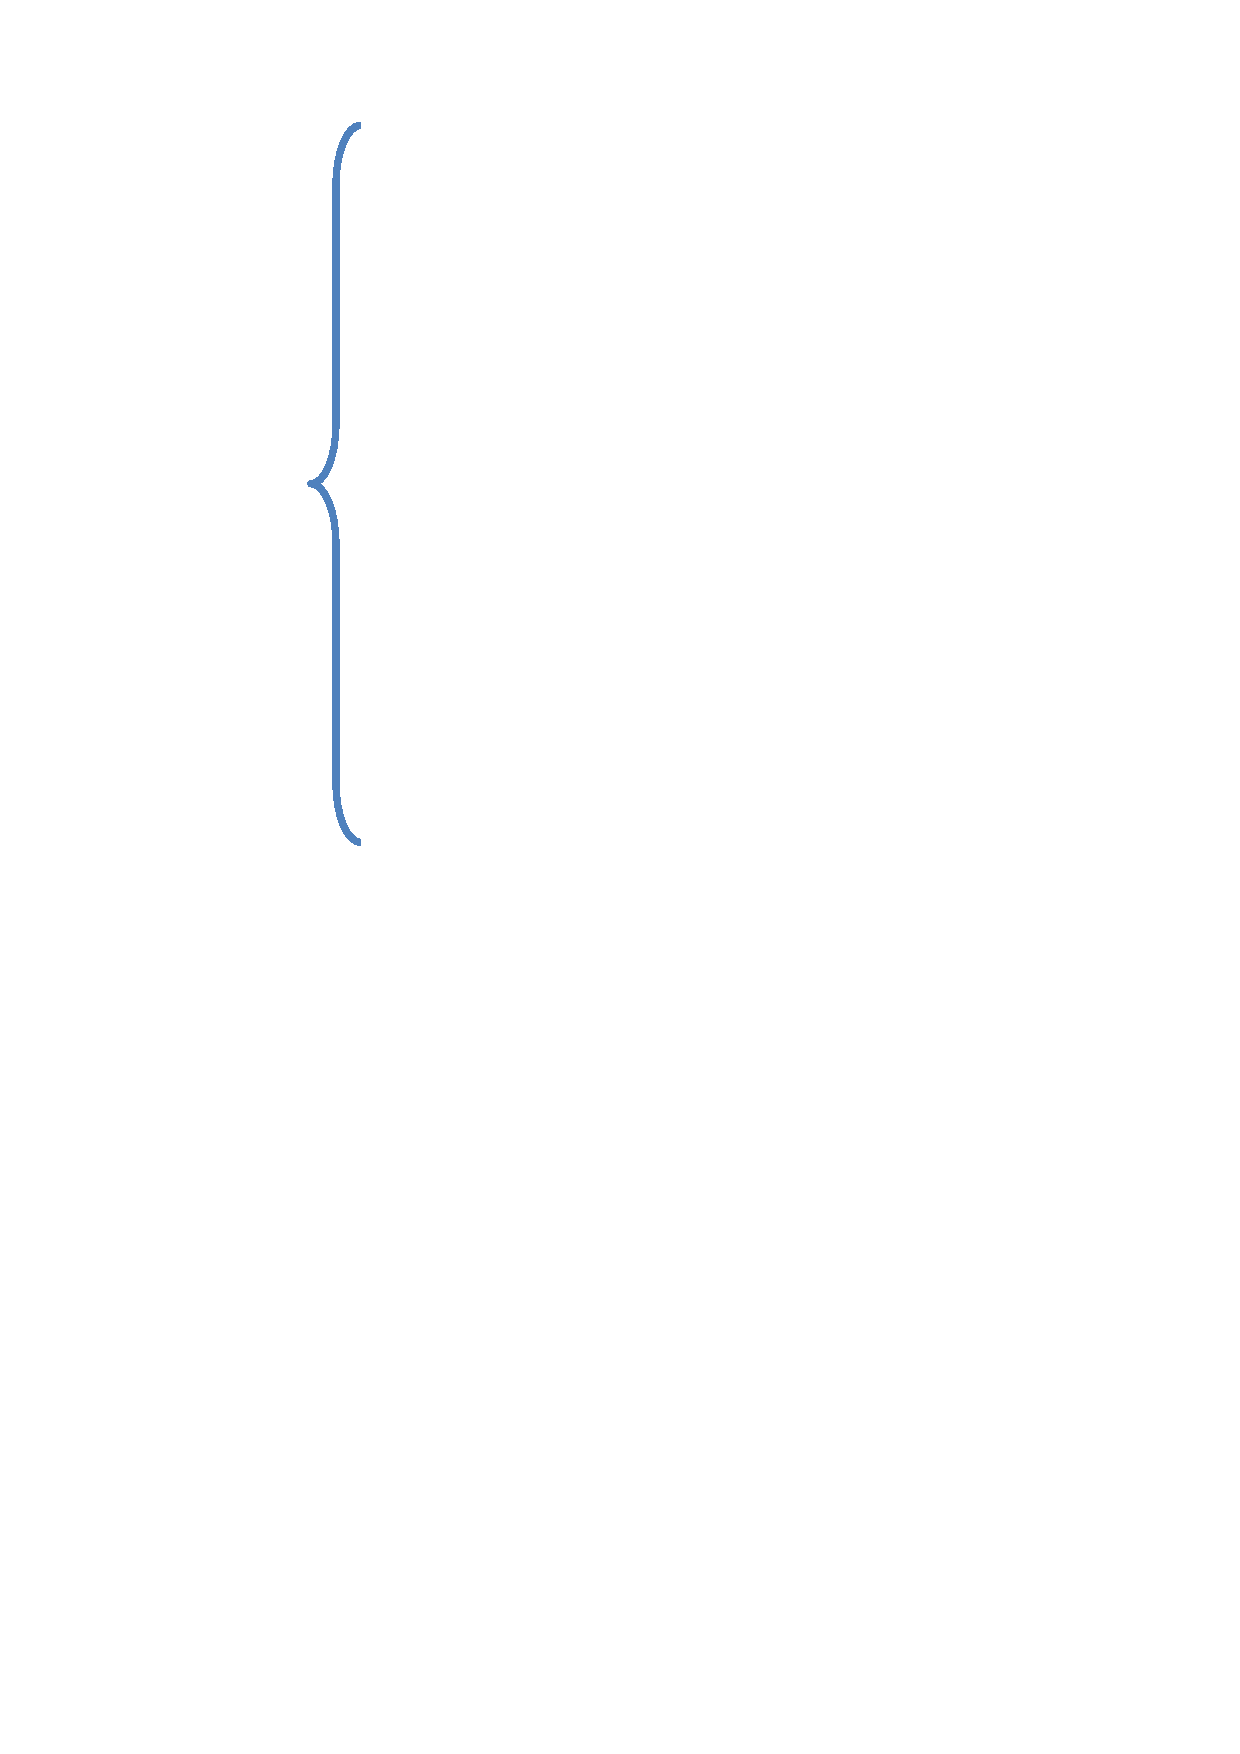
\includegraphics[width = 0.4cm, height = 2.2cm]{llave.pdf}
\end{column}
\begin{column}{4cm}
\vspace{-0.35cm}
\[
\frac{{\rm d}^4 u}{{\rm d} x^4} + u^2 \frac{{\rm d} u}{{\rm d} x} = {\rm cos} \, x
\]
\vspace{-0.2cm}
\[
\frac{\partial u}{\partial t} - \frac{\partial^2 u}{\partial x^2} - \frac{\partial^2 u}{\partial y^2} + u = 0.
\]
\end{column}
\begin{column}{3cm}
\end{column}
\end{columns}
%\vspace{0.1cm}
\textcolor{azul}{NOTACI\'{O}N:}
Hay dos notaciones muy comunes para las derivadas parciales que emplearemos a lo largo del curso:
\begin{itemize}
\item \textcolor{azul}{La notaci\'on de Leibnitz}, que es la usada en los
ejemplos anteriores.
\item Otra notaci\'{o}n mucho \textcolor{azul}{m\'{a}s compacta}, que emplea sub\'{\i}ndices para indicar derivadas
parciales: $u_t - u_{xx} - u_{yy} + u = 0.$
\end{itemize}
\vspace{-0.2cm}
\begin{block}{}{
Una ecuaci\'on diferencial es \textcolor{blue}{ordinaria (EDO)} si la funci\'on $u$ s\'olo depende de una variable, mientras que es \textcolor{blue}{parcial (EDP)} si depende de m\'as de una variable.}
\end{block}
\end{frame}

%%%%%%%%%%%%%%%%%%%%%%%%%%%%%%%%%%%%%%%%%%%%%%%%%%%%%%%%%%%%%%%%%%%%%%%%%%%%%%

\begin{frame}
\frametitle{Definici\'on de ecuaci\'on en derivadas parciales}
\small
\vspace{-0.2cm}
\begin{block}{Definici\'on}{
Una \textcolor{blue}{ecuaci\'on en derivadas parciales (EDP)} es una relaci\'on de la forma
\[
F(x,t,u,\frac{\partial u}{\partial x_1},\ldots,\frac{\partial u}{\partial x_n},\frac{\partial u}{\partial t}, \ldots, D^{\alpha} u) = 0
\]
}
donde la inc\'ognita $u=u({\mathbf x},t)$ es una funci\'on de la variable espacial ${\mathbf x}=(x_1, \ldots, x_n) \in \R^n$, y de
la variable temporal $t$.
\end{block}
\begin{itemize}
\item \textcolor{azul}{Notaci\'on de Schwartz}: $\alpha=(\alpha_0,\alpha_1, \ldots, \alpha_n) \in \R^{n+1}$ es un multi\'{\i}ndice de modo que \textcolor{azul}{$D^{\alpha} u$} denota una \textcolor{azul}{derivada parcial iterada} de u de orden $|\alpha| = \alpha_0+\alpha_1+ \ldots+\alpha_n$ en la que derivamos $\alpha_0$ veces con respecto a la variable $t$ y $\alpha_j$ veces con respecto a las variables $x_j, \;j = 1, \ldots, n.$
\item La inc\'{o}gnita \textcolor{azul}{$u$ representa una cantidad f\'{\i}sica}, como por ejemplo, temperatura, concentraci\'on de un contaminante, intensidad de una se\~{n}al ac\'ustica, deformaci\'on de una estructura, etc.
\end{itemize}
\end{frame}

%%%%%%%%%%%%%%%%%%%%%%%%%%%%%%%%%%%%%%%%%%%%%%%%%%%%%%%%%%%%%%%%%%%%%%%%

\begin{frame}
\frametitle{Ejemplos t\'{\i}picos de EDP's}
\small
\vspace{-0.4cm}
En los siguientes ejemplos se presentan algunas EDP's famosas que suelen llevar el nombre de su descubridor:\\ [2ex]

\includegraphics[width = 11cm,height = 5.8cm]{cuadro.pdf}
\vspace{-5.8cm}
\begin{itemize}
\item \textcolor{blue}{Ecuaci\'on de Laplace:} $u_{xx} + u_{yy} = 0.$
\vspace{0.15cm}
\item \textcolor{blue}{Ecuaci\'on de Fourier:} $u_{t} = u_{xx}.$
\vspace{0.15cm}
\item \textcolor{blue}{Ecuaci\'on de Euler-Bernoulli:} $u_{tt} = -\beta^2 u_{xxxx}.$
\vspace{0.15cm}
\item \textcolor{blue}{Ecuaci\'on de Schr\"{o}dinger:} $u_{t} = i \beta u_{xx}.$
\vspace{0.15cm}
\item \textcolor{blue}{Ecuaci\'on de Helmholtz:} $u_{xx} + u_{yy} + \alpha^2 u = 0.$
\vspace{0.15cm}
\item \textcolor{blue}{Ecuaci\'on de Korteweg-de Vries:} $u_{t} + \alpha u u_x + \beta u_{xxx} = 0.$
\end{itemize}
\end{frame}

%%%%%%%%%%%%%%%%%%%%%%%%%%%%%%%%%%%%%%%%%%%%%%%%%%%%%%%%%%%%%%%%%%%%%%%%

\begin{frame}
\frametitle{Orden de una ecuaci\'on en derivadas parciales}
\small
\vspace{-0.3cm}
\begin{block}{Definici\'on de orden}{
El \textcolor{blue}{orden} de una ecuaci\'on en derivadas parciales es el orden de la derivada
m\'as alta que aparece en la ecuaci\'on, es decir, el m\'aximo de los m\'odulos
$\alpha$ de los \'{\i}ndices que intervienen.
}
\end{block}
\vspace{0.1cm}

\includegraphics[width = 11cm, height = 2.1cm]{cuadro.pdf}
\vspace{-2.1cm}
\begin{columns}
\begin{column}{1cm}
\end{column}
\begin{column}{9cm}
\textcolor{blue}{La ecuaci\'on de transporte}:\\ [2ex]
$\quad \displaystyle\frac{\partial u}{\partial t} + a \frac{\partial u}{\partial x}  = 0\quad \quad$
es una ecuaci\'on de \textcolor{blue}{primer orden}.
\end{column}
\begin{column}{1cm}
\end{column}
\end{columns}
\vspace{0.4cm}

\includegraphics[width = 11cm, height = 2.1cm]{cuadro.pdf}
\vspace{-2.1cm}
\begin{columns}
\begin{column}{1cm}
\end{column}
\begin{column}{9cm}
\textcolor{blue}{La ecuaci\'on del calor}:\\ [2ex]
$\quad \displaystyle\frac{\partial u}{\partial t} - \frac{\partial^2 u}{\partial x^2}  = 0\quad \quad$
es una ecuaci\'on de \textcolor{blue}{segundo orden}.
\end{column}
\begin{column}{1cm}
\end{column}
\end{columns}
\vspace{0.7cm}
En este curso nos limitaremos al estudio de EDP's de primer y segundo orden.
\end{frame}

%%%%%%%%%%%%%%%%%%%%%%%%%%%%%%%%%%%%%%%%%%%%%%%%%%%%%%%%%%%%%%%%%%%%%%%%

\begin{frame}
\frametitle{Soluci\'on cl\'asica}
\small
\vspace{-0.1cm}
\begin{block}{Definici\'on de soluci\'{o}n cl\'{a}sica}{
Se llama \textcolor{blue}{soluci\'on cl\'asica} de una ecuaci\'on en derivadas parciales de orden $m$
en un abierto $\Omega \subset \R^n$, a una funci\'on $u \in C^m(\Omega)$ tal que sustituyendo esta funci\'on
y sus derivadas en la ecuaci\'on
\[
F(x,t,u,\frac{\partial u}{\partial x_1},\ldots,\frac{\partial u}{\partial x_n}, \ldots, D^{\alpha} u) = 0
\]
se obtiene una identidad.
}
\end{block}
\vspace{-0.1cm}
\begin{itemize}
\item En la definici\'on anterior no se especifica la \textcolor{azul}{regularidad de la soluci\'on en la frontera $\partial \Omega$}. Generalmente se pide que la funci\'on sea continua en  $\partial \Omega$.
\item La definici\'on caracteriza las soluciones como aquellas funciones de clase $C^m(\Omega)$ que satisfacen la ecuaci\'on en todo punto de $\Omega$. A este tipo de soluciones se les llama \textcolor{blue}{soluciones cl\'asicas o fuertes.} Se puede demostrar la existencia de \textcolor{blue}{soluciones d\'ebiles} que satisfacen la ecuaci\'on en casi todo punto (\textcolor{blue}{teor\'{\i}a de distribuciones}).
\end{itemize}
\end{frame}

%%%%%%%%%%%%%%%%%%%%%%%%%%%%%%%%%%%%%%%%%%%%%%%%%%%%%%%%%%%%%%%%%%%%%%%%

\begin{frame}
\frametitle{Ejemplo de soluci\'on cl\'asica}
\small
\begin{block}{La ecuaci\'on del calor}{
\[
\frac{\partial u}{\partial t} - \frac{\partial^2 u}{\partial x^2}  = 0.
\]
Una soluci\'on cl\'asica de la ecuaci\'on del calor es una funci\'on $u(x,t)$ definida en un dominio $\Omega \subset \R^2$
tal que
\begin{itemize}
\item $u\in C^2(\Omega)$
\item $u$ satisface la ecuaci\'on $u_t=u_{xx}$ en todo punto de $\Omega.$
\end{itemize}}
\end{block}
\vspace{0.2cm}
Por ejemplo:
\begin{itemize}
\item $u(x,t) = t + x^2/2$ es una soluci\'on cl\'asica de la ecuaci\'on del calor en $\Omega=\R^2$.
\item $\displaystyle u(x,t) = \frac{{\rm e}^{-x^2/4t}}{2 \sqrt{\pi \, t}}$ es una soluci\'on cl\'asica de la ecuaci\'on del calor en
$\Omega = \{(x,t), t>0\} \subset \R^2$.
\end{itemize}
\end{frame}

%%%%%%%%%%%%%%%%%%%%%%%%%%%%%%%%%%%%%%%%%%%%%%%%%%%%%%%%%%%%%%%%%%%%%%%%

\begin{frame}
\frametitle{Ejemplo de resoluci\'on de una EDP}
\small
\vspace{-0.5cm}
\begin{columns}
\begin{column}{1cm}
\end{column}
\begin{column}{9cm}
\begin{block}{}{
\begin{center}\textcolor{azul}{El proceso de resoluci\'on de una EDP se llama tambi\'en} \\ \textcolor{blue}{integraci\'on} \textcolor{azul}{de la EDP}
\end{center}}
\end{block}
\end{column}
\begin{column}{1cm}
\end{column}
\end{columns}
\vspace{0.3cm}
En algunos casos la resoluci\'on de una ecuaci\'on en derivadas parciales es directa, entendiendo
por ello que se realiza mediante integraci\'on directa.
\begin{block}{Ejemplo: Resolver la ecuaci\'on $\displaystyle \frac{\partial u}{\partial x} = x + y$}{
Se trata evidentemente de una EDP de primer orden. Buscamos una soluci\'on $u(x,y)$ de clase $C^1$.
Integrando directamente respecto a $x$, obtenemos
\[
u(x,y) = xy + \frac{x^2}{2} + f(y),
\]
donde $f(y)$ es una funci\'on derivable arbitraria de $y$.
}
\end{block}
En el ejemplo anterior hemos obtenido infinitas soluciones de la EDP. A la expresi\'on obtenida
se le llama \textcolor{blue}{soluci\'on general.}
\end{frame}

%%%%%%%%%%%%%%%%%%%%%%%%%%%%%%%%%%%%%%%%%%%%%%%%%%%%%%%%%%%%%%%%%%%%%%%%%%%%%%%%

\begin{frame}
\frametitle{Condiciones iniciales y de contorno}
\small
\vspace{-0.2cm}
\begin{columns}
\begin{column}{1.5cm}
\end{column}
\begin{column}{8.5cm}
\begin{block}{}{
\begin{center}Una EDP en general tendr\'a \textcolor{blue}{infinitas soluciones}\end{center}}
\end{block}
\end{column}
\begin{column}{1.5cm}
\end{column}
\end{columns}
\vspace{0.1cm}

\includegraphics[width = 11cm, height = 3.6cm]{cuadro.pdf}
\vspace{-3.1cm}
\begin{columns}
\begin{column}{1cm}
\end{column}
\begin{column}{10cm}
Para describir completamente el proceso f\'{\i}sico hace falta plantear:
\begin{itemize}
\item el \textcolor{blue}{estado inicial} del proceso\\ (las \textcolor{azul}{CONDICIONES INICIALES} para problemas de evoluci\'on)
\item el \textcolor{blue}{r\'egimen en la frontera $\partial \Omega$} de la regi\'on $\Omega$ donde tiene lugar el proceso (las \textcolor{azul}{CONDICIONES DE CONTORNO})
\end{itemize}
\end{column}
\begin{column}{1cm}
\end{column}
\end{columns}
\vspace{0.5cm}
\begin{itemize}
\item En EDP's que modelan \textcolor{blue}{procesos de equilibrio}, la EDP debe de ser suplementada por \textcolor{blue}{condiciones de contorno} adecuadas.
\item En EDP's que modelan \textcolor{blue}{procesos din\'amicos} (en los que el tiempo es una de las variables independientes) hay que especificar una o m\'{a}s \textcolor{blue}{condiciones iniciales}.\\
    Este n\'umero viene dado por la derivada de mayor orden con respecto al tiempo que aparece en la ecuaci\'on.
\end{itemize}
\end{frame}

%%%%%%%%%%%%%%%%%%%%%%%%%%%%%%%%%%%%%%%%%%%%%%%%%%%%%%%%%%%%%%%%%%%%%%%%%%%%%%%%%%%%%%%%%%%

\begin{frame}
\frametitle{Tipos de condiciones de contorno}
\small
Hay principalmente tres tipos de condiciones de contorno:
\vspace{0.1cm}
\begin{columns}
\begin{column}{0.5cm}
\end{column}
\begin{column}{0.5cm}
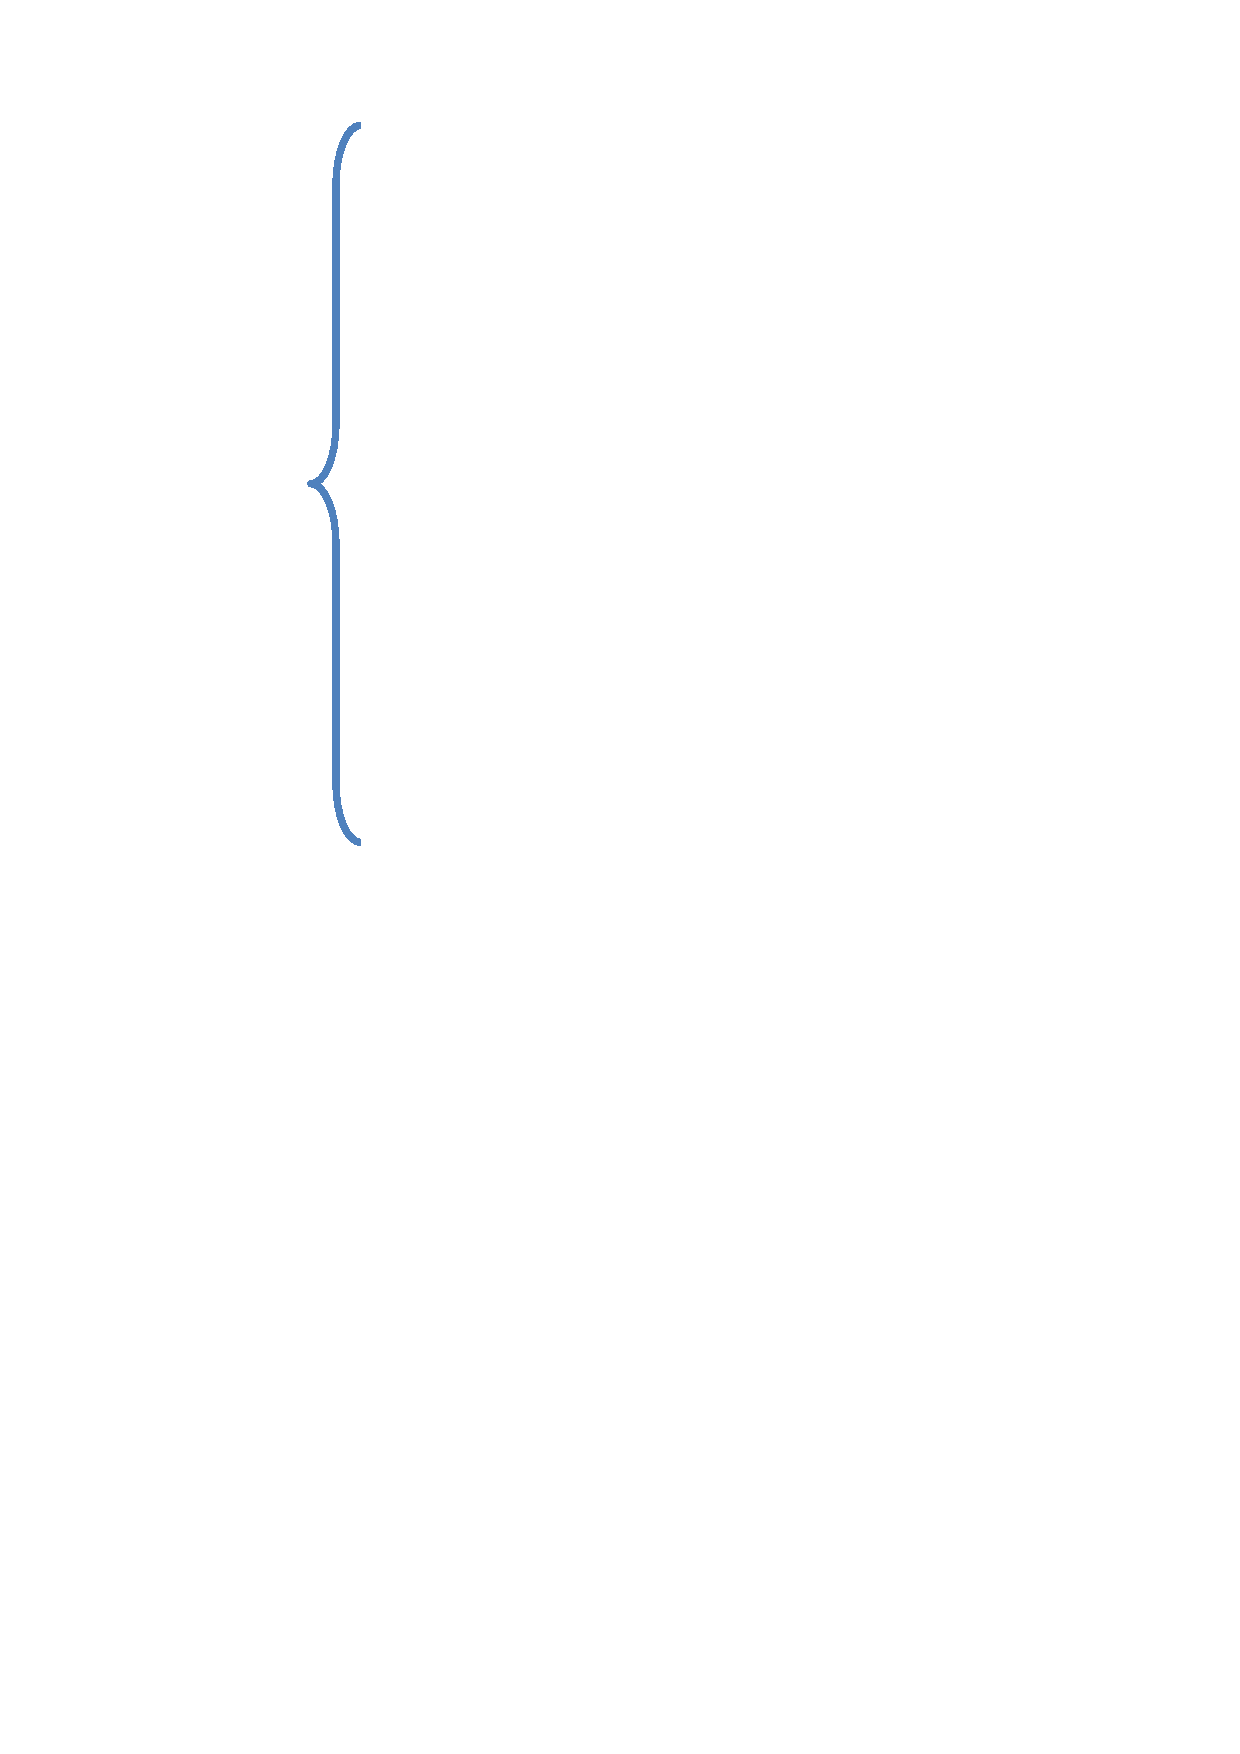
\includegraphics[width = 0.5cm, height = 7.5cm]{llave.pdf}
\end{column}
\hspace{-0.4cm}
\begin{column}{11cm}
\vspace{-0.5cm}
\begin{itemize}
\item \textcolor{blue}{Condici\'on de tipo Dirichlet}. Consiste en \textcolor{azul}{especificar la funci\'on en la frontera del dominio}.\\ [0.6ex]
    Por ejemplo, en un problema de equilibrio t\'ermico, la condici\'on de contorno especifica la temperatura en el contorno y nuestro objetivo ser\'a encontrar la distribuci\'on de la temperatura en el interior.
\item \textcolor{blue}{Condici\'on de tipo Neumann}. Consiste en \textcolor{azul}{especificar la derivada normal de la funci\'on en la frontera del dominio}. \\ [0.6ex]
    En el ejemplo del equilibrio t\'ermico, esta condici\'on prescribe el flujo de calor que atraviesa la frontera, que por la ley de Fourier es proporcional al gradiente de temperatura. En particular un contorno aislado no tiene flujo, y por tanto, la derivada normal es cero en dicho contorno.
\item \textcolor{blue}{Condici\'on de tipo Robin o mixto}. Este tipo de condiciones se usa para expresar que el flujo de calor es proporcional a la diferencia de temperaturas entre el contorno y el exterior del dominio.
\end{itemize}
\end{column}
\begin{column}{1.5cm}
\end{column}
\end{columns}
\end{frame}

%%%%%%%%%%%%%%%%%%%%%%%%%%%%%%%%%%%%%%%%%%%%%%%%%%%%%%%%%%%%%%%%%%%%%%%%%%%%%%%%%%%%%%%%%%%

\begin{frame}
\frametitle{Sistema de ecuaciones en derivadas parciales}
\small
\vspace{-0.3cm}
\begin{block}{Definici\'on}{
Un \textcolor{blue}{sistema de ecuaciones en derivadas parciales} es un conjunto de una o m\'as ecuaciones que relacionan las derivadas de una o m\'{a}s funciones. \\ [0.5ex]
El \textcolor{blue}{orden del sistema} es el orden de la derivada m\'as alta que aparece en dichas ecuaciones.
}\end{block}
\vspace{0.1cm}
\begin{columns}
\begin{column}{0.2cm}
\end{column}
\begin{column}{0.5cm}
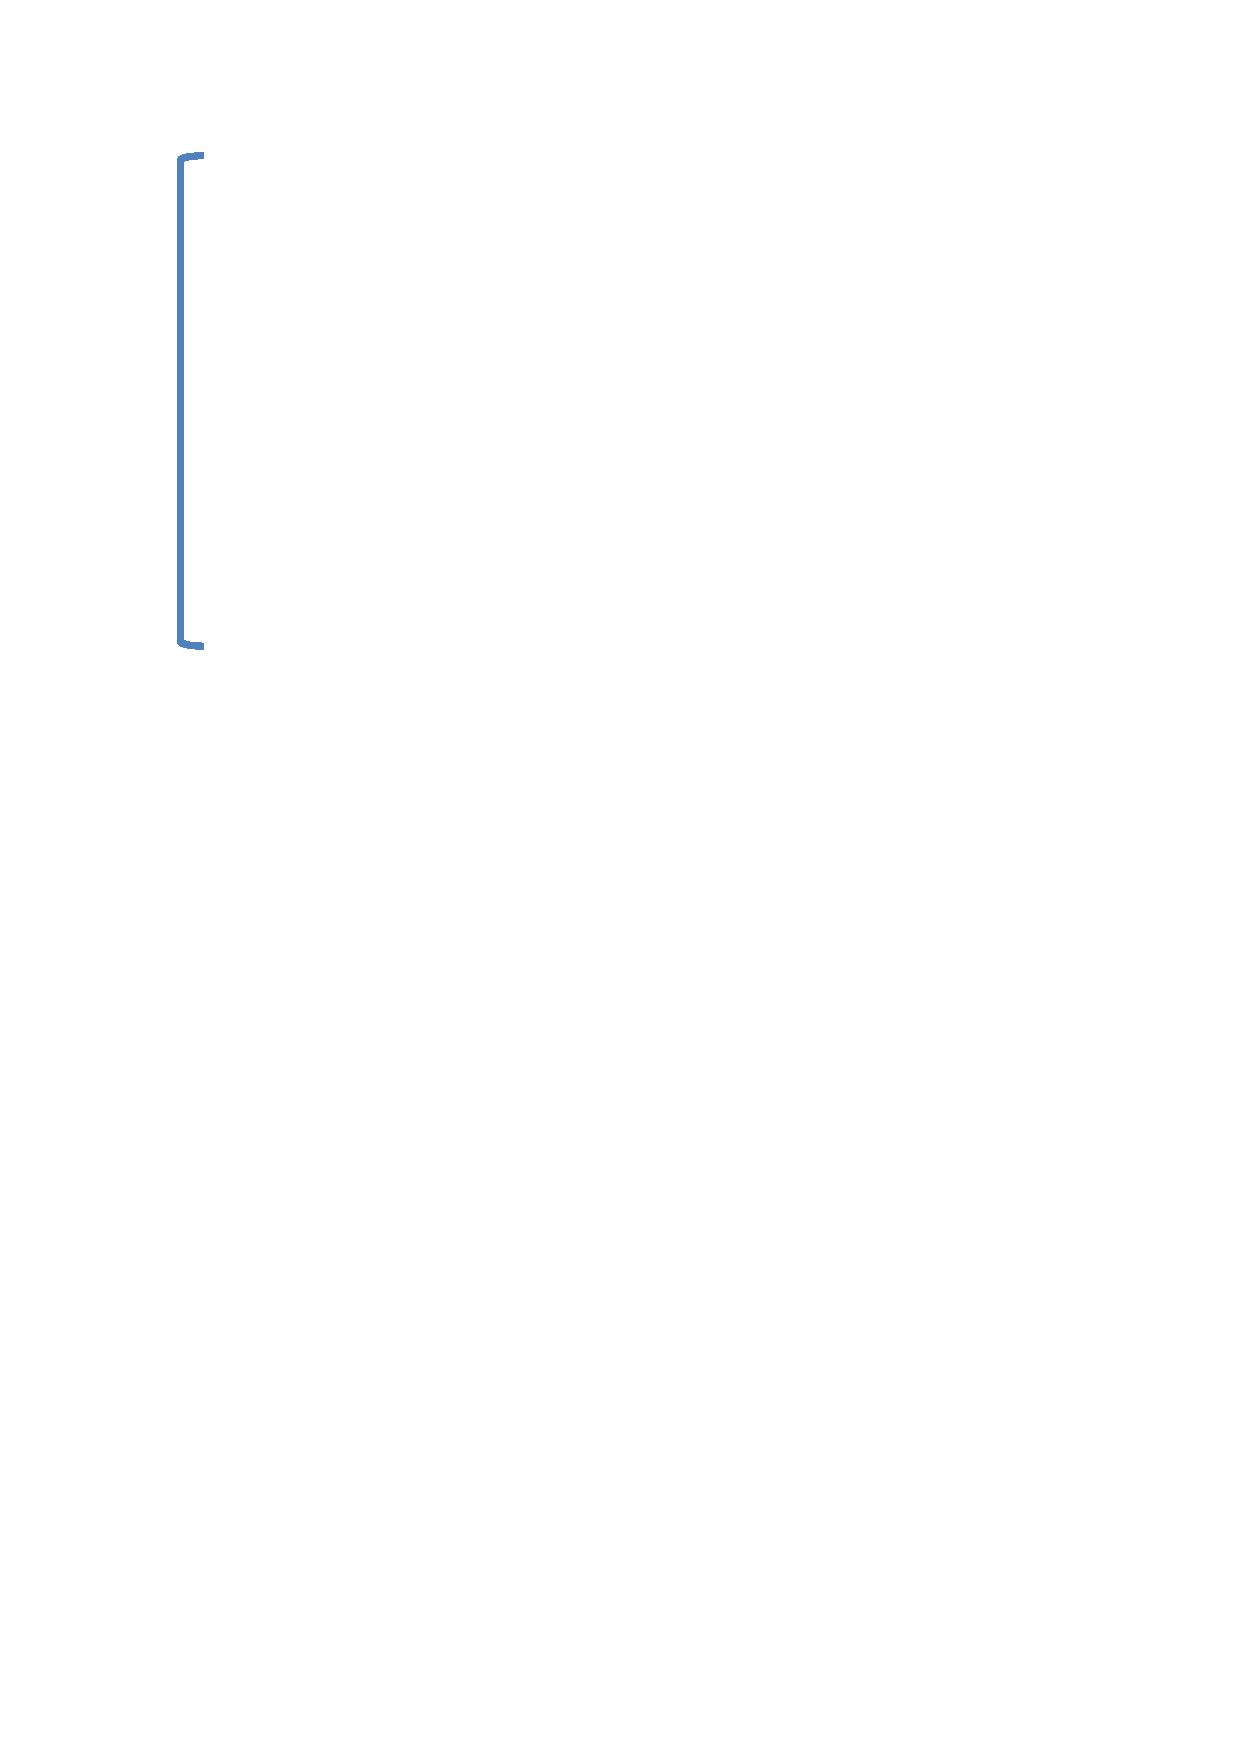
\includegraphics[width = 0.6cm, height = 4cm]{corchete.pdf}
\end{column}
\hspace{-0.3cm}
\begin{column}{10cm}
\textbf{EJEMPLO:} Las \textcolor{azul}{ecuaciones de Navier-Stokes} en tres dimensiones:
\begin{eqnarray}
& & \frac{\partial u}{\partial t} + u \frac{\partial u}{\partial x} + v \frac{\partial u}{\partial y} + w \frac{\partial u}{\partial z} -
\nu \left(\frac{\partial^2 u}{\partial x^2} + \frac{\partial^2 u}{\partial y^2} + \frac{\partial^2 u}{\partial z^2}\right) + \frac{\partial p}{\partial x} = 0, \nonumber \\
& & \frac{\partial v}{\partial t} + u \frac{\partial v}{\partial x} + v \frac{\partial v}{\partial y} + w \frac{\partial v}{\partial z} -
\nu \left(\frac{\partial^2 v}{\partial x^2} + \frac{\partial^2 v}{\partial y^2} + \frac{\partial^2 v}{\partial z^2}\right) + \frac{\partial p}{\partial y} = 0, \nonumber \\
& & \frac{\partial w}{\partial t} + u \frac{\partial w}{\partial x} + v \frac{\partial w}{\partial y} + w \frac{\partial w}{\partial z} -
\nu \left(\frac{\partial^2 w}{\partial x^2} + \frac{\partial^2 w}{\partial y^2} + \frac{\partial^2 w}{\partial z^2}\right) + \frac{\partial p}{\partial z} = 0, \nonumber
\end{eqnarray}
\end{column}
\begin{column}{1cm}
\end{column}
\end{columns}
\vspace{0.1cm}
La existencia y unicidad de soluci\'on es uno de los problemas del milenio
\vspace{-0.2cm}
\begin{center}\textcolor{blue}{http://www.claymath.org}\end{center}
\end{frame}



%%%%%%%%%%%%%%%%%%%%%%%%%%%%%%%%%%%%%%%%%%%%%%%%%%%%%%%%%%%%%%%%%%%%%%%%%%%%%%%%%%%%%%%%%%%


\begin{frame}
\frametitle{Ejemplos cl\'asicos de EDP's lineales de segundo orden}
\small
\vspace{-0.5cm}
Finalmente, para terminar el primer tema dedicado a la introducci\'on a las EDP's vamos
a presentar los \textcolor{azul}{EJEMPLOS CL\'{A}SICOS} m\'as estudiados junto con las ecuaciones de primer orden.\\ [0.5ex]
Son ecuaciones que tienen una gran importancia dentro de la f\'{\i}sica debido a la gran variedad
de situaciones reales que responden a estos modelos matem\'{a}ticos.
\vspace{0.2cm}
\begin{columns}
\begin{column}{0.2cm}
\end{column}
\begin{column}{0.5cm}
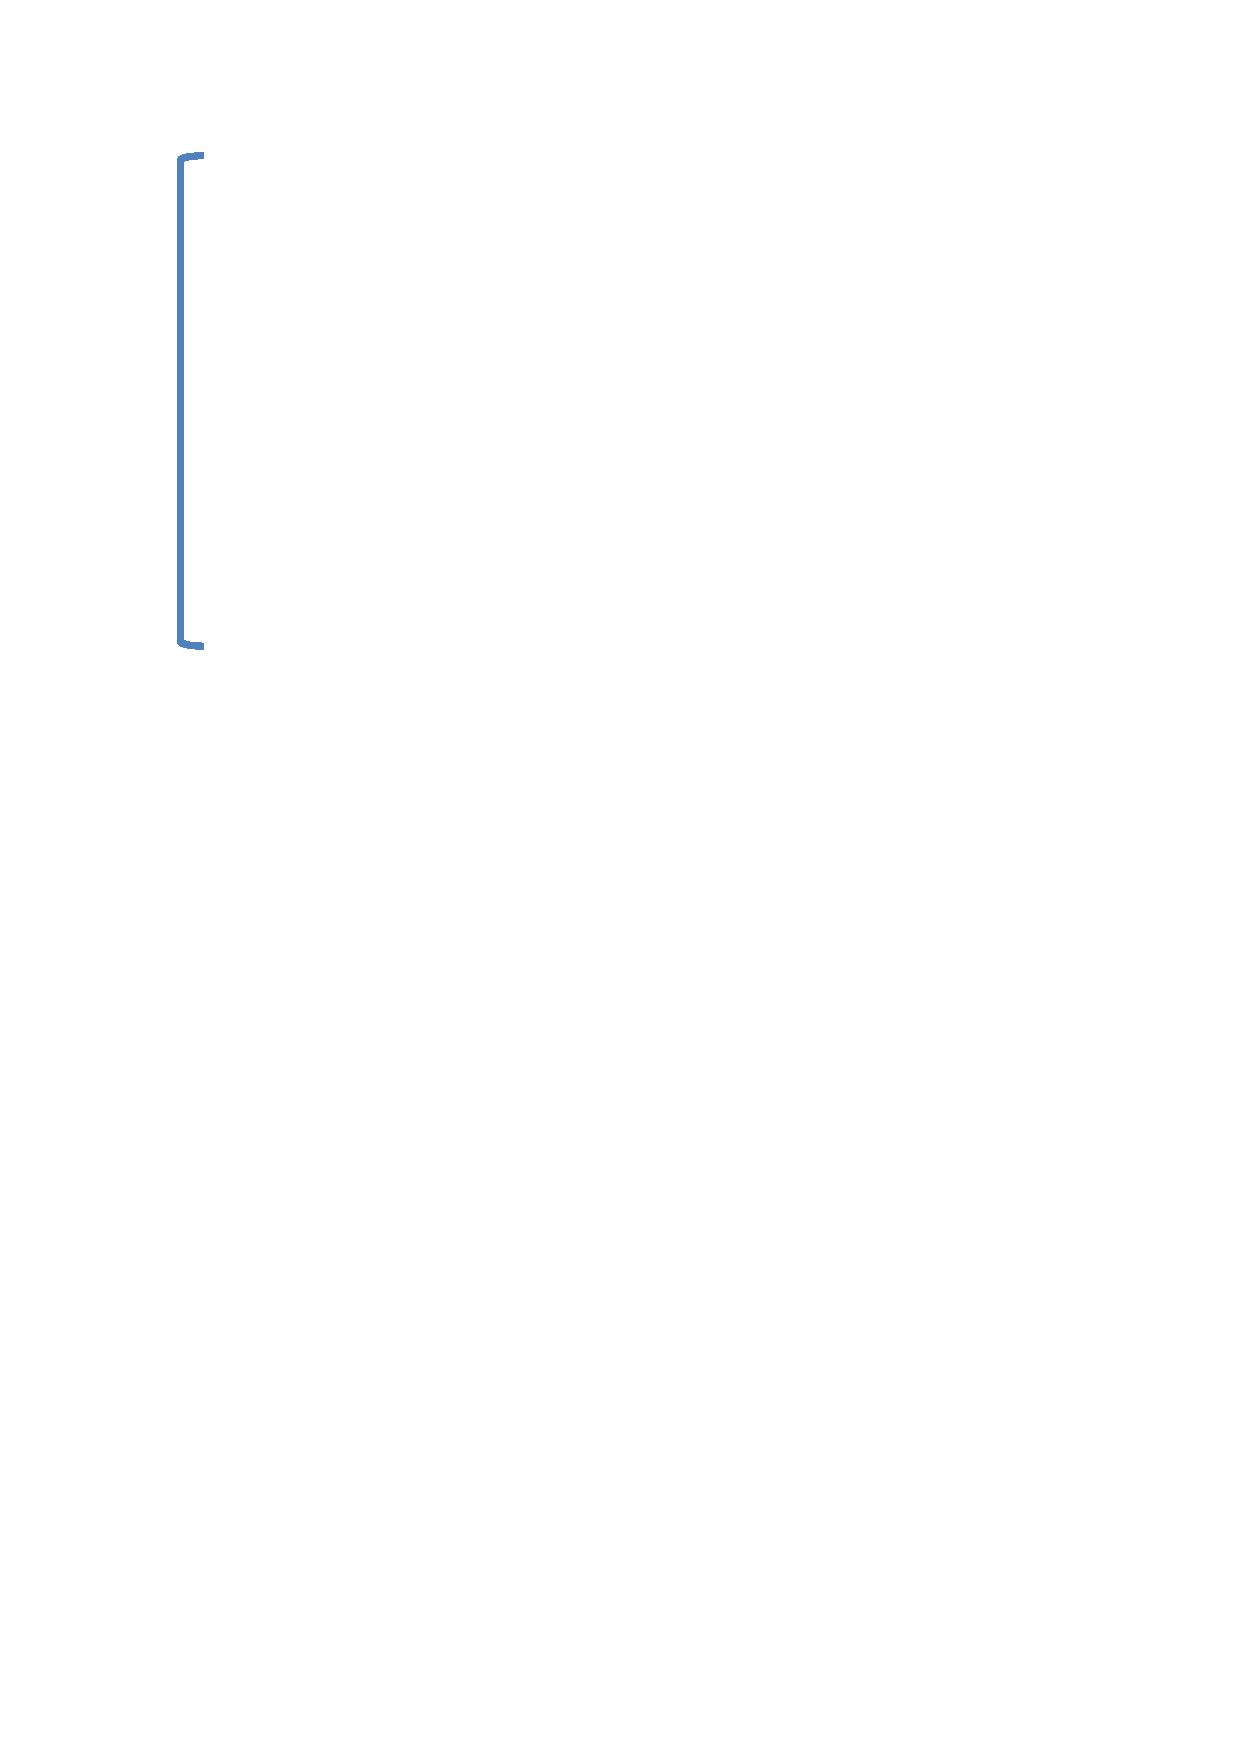
\includegraphics[width = 0.6cm, height = 3cm]{corchete.pdf}
\end{column}
\hspace{-0.3cm}
\begin{column}{10cm}
\begin{itemize}
\item \textcolor{blue}{Ecuaci\'on de Laplace:} $\quad\displaystyle - \Delta u = 0$.
\vspace{0.1cm}
\item \textcolor{blue}{Ecuaci\'on del calor:} $\quad\displaystyle \rho(x) \frac{\partial u}{\partial t} - \nabla \cdot (\kappa(x) \nabla u)= 0$
\vspace{0.1cm}
\item \textcolor{blue}{Ecuaci\'on de ondas:} $\quad\displaystyle \frac{1}{c^2} \frac{\partial^2 u}{\partial t^2} - \Delta u= f(x,t)$
\end{itemize}
\end{column}
\begin{column}{1cm}
\end{column}
\end{columns}
\end{frame}

%%%%%%%%%%%%%%%%%%%%%%%%%%%%%%%%%%%%%%%%%%%%%%%%%%%%%%%%%%%%%%%%%

\end{document}
